\documentclass[11pt,a4paper]{article}

\usepackage{amsmath,amssymb}
\usepackage[margin=2cm]{geometry}
\usepackage{enumitem}
\usepackage{tikz}
\usetikzlibrary{angles,quotes}

\setlength{\parindent}{0pt}
\setlength{\parskip}{4pt}
\setlength{\emergencystretch}{1.5em}
\setlist[enumerate,1]{label=\arabic*.,leftmargin=*,itemsep=0.7em}
\setlist[enumerate,2]{label=\alph*.,leftmargin=*,itemsep=0.3em,topsep=0.3em}
\newcommand{\vect}[1]{\overrightarrow{#1}}

\begin{document}

\begin{center}
    {\large\bfseries USULAN EVALUASI TENGAH SEMESTER (ETS)\\
    FISIKA MATEMATIKA 1}\\
    {\bfseries SEMESTER GASAL 2025/2026}\\
    {\bfseries INSTITUT TEKNOLOGI SEPULUH NOPEMBER}
\end{center}
\begin{tabular}{@{}ll@{}}
    Mata Kuliah  & : Fisika Matematika 1 \\
    Hari/Tanggal & : Senin, 13 Oktober 2025 (11.00--12.40 WIB) \\
    Waktu        & : 100 menit (\textbf{Kejujuran di atas segalanya})
\end{tabular}

\smallskip
\hrule
\medskip

\begin{enumerate}
    \item Tentukan luas segitiga yang disusun oleh titik-titik
    $P_1=(2,2,0)$, $P_2=(-1,0,2)$, $P_3=(0,4,3)$ dengan:
    \begin{enumerate}
        \item Perkalian silang (\textit{cross product}).
        \item Perkalian titik (\textit{dot product}).
    \end{enumerate}

    \item Tentukan persamaan bidang yang melalui ketiga buah titik
    berikut: $A=(-1,1,1)$, $B=(2,3,0)$, dan $C=(0,1,-2)$;
    serta tentukan persamaan garis yang melalui titik $D=(1,0,-2)$
    dan tegak lurus bidang tersebut, kemudian tentukan jarak titik
    tersebut ke bidangnya.

    \item Tentukan semua solusi yang mungkin dari persamaan berikut
    dengan menggunakan pendekatan Gauss--Jordan (reduksi baris):
    \begin{enumerate}
        \item
        \[
        \begin{aligned}
            2x-z&=2,\\
            6x+5y+3z&=7,\\
            2x-y&=4.
        \end{aligned}
        \]
        \item
        \[
        \begin{aligned}
            x_1+2x_2+3x_3&=0,\\
            2x_1+5x_2+3x_3&=0,\\
            x_1+8x_3&=0.
        \end{aligned}
        \]
    \end{enumerate}

    \item Diketahui matriks
    \[
        A=\begin{pmatrix}
            1&\sqrt{2}\\
            -\sqrt{2}&1
        \end{pmatrix}
        \quad\text{dan}\quad
        B=\begin{pmatrix}
            1&\sqrt{2}\\
            -\sqrt{2}&k
        \end{pmatrix}.
    \]
    Tentukan:
    \begin{enumerate}
        \item Apakah mungkin menemukan nilai $k$ sehingga $AB=BA$?
        Jika ya, berapakah nilai $k$ tersebut?
        \item $A^3$.
    \end{enumerate}
\end{enumerate}

\newpage

\begin{center}
    {\Large\bfseries Pembahasan}
\end{center}

\begin{enumerate}
\item
Ambil dua vektor sisi segitiga yang berpangkal di $P_1$:
\begin{align*}
    \mathbf{u}=\vect{P_1P_2}&=P_2-P_1=(-3,-2,2),\\
    \mathbf{v}=\vect{P_1P_3}&=P_3-P_1=(-2,2,3).
\end{align*}

\begin{enumerate}
\item

Luas segitiga adalah setengah luas jajargenjang yang dibentuk oleh
$\mathbf{u}$ dan $\mathbf{v}$. Pada gambar, diagonal $P_2P_3$
membagi jajargenjang $P_1P_2QP_3$ menjadi dua segitiga sama luas.
\begin{center}
    \begin{tikzpicture}[line width=0.4pt]
        \coordinate (P1) at (0,0);
        \coordinate (P2) at (4.25,0);
        \coordinate (P3) at (2,3.75);
        \coordinate (Q) at (6.25,3.75);
        \draw (P1) -- node[midway,below] {$\mathbf{u}$} (P2)
                   -- (P3)
                   -- node[midway,left=2pt] {$\mathbf{v}$} (P1);
        \draw[densely dashed] (P2) -- (Q) -- (P3);
        \pic[draw,"$\theta$",angle radius=6mm,
             angle eccentricity=0.6,font=\small]
            {angle=P2--P1--P3};
        \node[below left] at (P1) {$P_1$};
        \node[below right] at (P2) {$P_2$};
        \node[above] at (P3) {$P_3$};
        \node[above] at (Q) {$Q$};
    \end{tikzpicture}
\end{center}
Karena $\|\mathbf{u}\times\mathbf{v}\|$ adalah luas jajargenjang,
\[
    L=\frac12\|\mathbf{u}\times\mathbf{v}\|.
\]
Hasil perkalian silangnya adalah
\begin{align*}
    \mathbf{u}\times\mathbf{v}
    &=\begin{vmatrix}
        \mathbf{i}&\mathbf{j}&\mathbf{k}\\
        -3&-2&2\\
        -2&2&3
    \end{vmatrix}\\
    &=\bigl((-2)(3)-(2)(2),\;
            (2)(-2)-(-3)(3),\;
            (-3)(2)-(-2)(-2)\bigr)\\
    &=(-10,5,-10).
\end{align*}
Dengan demikian,
\[
    L=\frac12\sqrt{(-10)^2+5^2+(-10)^2}
     =\frac12\sqrt{225}
     =\boxed{\frac{15}{2}\text{ satuan luas}}.
\]

\item

Panjang kedua sisi dan perkalian titiknya adalah
\begin{align*}
    \|\mathbf{u}\|&=\sqrt{(-3)^2+(-2)^2+2^2}=\sqrt{17},\\
    \|\mathbf{v}\|&=\sqrt{(-2)^2+2^2+3^2}=\sqrt{17},\\
    \mathbf{u}\cdot\mathbf{v}&=(-3)(-2)+(-2)(2)+(2)(3)=8.
\end{align*}
Untuk sudut $\theta$ antara $\mathbf{u}$ dan $\mathbf{v}$, hubungan
$\mathbf{u}\cdot\mathbf{v}=\|\mathbf{u}\|\,\|\mathbf{v}\|\cos\theta$
memberikan
\[
    \cos\theta=\frac{\mathbf{u}\cdot\mathbf{v}}
                     {\|\mathbf{u}\|\,\|\mathbf{v}\|}
              =\frac8{\sqrt{17}\sqrt{17}}=\frac8{17}.
\]
Gunakan segitiga siku-siku bantu dengan perbandingan sisi samping
dan sisi miring $8:17$ untuk menentukan $\sin\theta$.
\begin{center}
    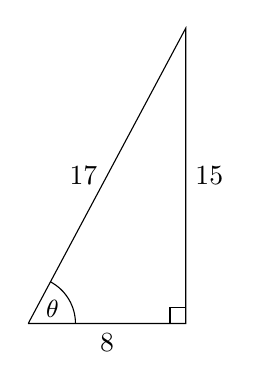
\begin{tikzpicture}[line width=0.4pt]
        \coordinate (O) at (0,0);
        \coordinate (A) at (2,0);
        \coordinate (B) at (2,3.75);
        \draw (O) -- node[midway,below] {$8$} (A)
                  -- node[midway,right] {$15$} (B)
                  -- node[midway,left] {$17$} (O);
        \pic[draw,angle radius=2mm] {right angle=B--A--O};
        \pic[draw,"$\theta$",angle radius=6mm,
             angle eccentricity=0.6,font=\small]
            {angle=A--O--B};
    \end{tikzpicture}
\end{center}
Dengan Teorema Pythagoras, sisi di depan $\theta$ adalah
$\sqrt{17^2-8^2}=15$, sehingga
\[
    \sin\theta=\frac{\text{sisi depan}}{\text{sisi miring}}
              =\frac{15}{17}.
\]
Segitiga semula memiliki alas $\|\mathbf{u}\|$ dan tinggi
$\|\mathbf{v}\|\sin\theta$, maka luasnya
\[
    L=\frac12\|\mathbf{u}\|\,\|\mathbf{v}\|\sin\theta
     =\frac12\,\sqrt{17}\cdot\sqrt{17}\cdot\frac{15}{17}
     =\boxed{\frac{15}{2}\text{ satuan luas}}.
\]
\end{enumerate}

\item
Dua vektor arah pada bidang adalah
\[
    \vect{AB}=B-A=(3,2,-1),\qquad
    \vect{AC}=C-A=(1,0,-3).
\]
Perkalian  silangnya memberikan vektor normal:
\[
    \vect{AB}\times\vect{AC}
    =\begin{vmatrix}
        \mathbf{i}&\mathbf{j}&\mathbf{k}\\
        3&2&-1\\
        1&0&-3
    \end{vmatrix}
    =(-6,8,-2).
\]
Pilih normal yang lebih sederhana, yaitu $\mathbf{n}=(3,-4,1)$.
Karena bidang melalui $A=(-1,1,1)$, persamaannya memenuhi
\begin{align*}
    \mathbf{n}\cdot\bigl((x,y,z)-A\bigr)&=0,\\
    3(x+1)-4(y-1)+(z-1)&=0.
\end{align*}
Jadi persamaan bidangnya adalah
\[
    \boxed{3x-4y+z+6=0}.
\]
Pemeriksaan pada ketiga titik memberikan
\[
    3(-1)-4(1)+1+6=0,\quad
    3(2)-4(3)+0+6=0,\quad
    3(0)-4(1)-2+6=0.
\]

Garis yang tegak lurus bidang mempunyai vektor arah sejajar dengan
normal $\mathbf{n}=(3,-4,1)$. Karena melalui $D=(1,0,-2)$,
persamaan garisnya adalah
\[
    \boxed{(x,y,z)=(1,0,-2)+t(3,-4,1),\qquad t\in\mathbb{R}}.
\]
Dalam bentuk parametrik,
\[
    \boxed{x=1+3t,\qquad y=-4t,\qquad z=-2+t}.
\]

Jarak titik $(x_0,y_0,z_0)$ ke bidang $ax+by+cz+d_0=0$ adalah
\[
    d=\frac{|ax_0+by_0+cz_0+d_0|}{\sqrt{a^2+b^2+c^2}}.
\]
Dengan memasukkan $D=(1,0,-2)$, diperoleh
\[
    d=\frac{|3(1)-4(0)+(-2)+6|}{\sqrt{3^2+(-4)^2+1^2}}
     =\boxed{\frac{7}{\sqrt{26}}\text{ satuan panjang}}.
\]
Sebagai pemeriksaan, substitusi persamaan garis ke persamaan bidang
menghasilkan
\[
    3(1+3t)-4(-4t)+(-2+t)+6=0
    \quad\Longrightarrow\quad t=-\frac7{26}.
\]
Kaki tegak lurus dari $D$ ke bidang adalah
\[
    H=D-\frac7{26}\mathbf{n}
     =\left(\frac5{26},\frac{14}{13},-\frac{59}{26}\right).
\]
Dengan demikian,
\[
    \|D-H\|=\left\|\frac7{26}\mathbf{n}\right\|
           =\frac7{26}\sqrt{26}
           =\frac7{\sqrt{26}}.
\]

\item
Pada reduksi berikut, $B_i$ menyatakan baris ke-$i$ dari matriks
diperbesar. Operasi baris elementer digunakan sampai bagian koefisien
menjadi matriks identitas.

\begin{enumerate}
\item
Matriks diperbesar untuk sistem pertama direduksi dengan menghilangkan
elemen di bawah pivot pertama:
\[
    \left(\begin{array}{ccc|c}
        2&0&-1&2\\
        6&5&3&7\\
        2&-1&0&4
    \end{array}\right)
    \xrightarrow{\substack{B_2\leftarrow B_2-3B_1\\
                            B_3\leftarrow B_3-B_1}}
    \left(\begin{array}{ccc|c}
        2&0&-1&2\\
        0&5&6&1\\
        0&-1&1&2
    \end{array}\right).
\]
Tukar $B_2$ dengan $B_3$, lalu kalikan baris kedua dengan $-1$.
Selanjutnya hilangkan elemen di bawah pivot kedua:
\[
    \left(\begin{array}{ccc|c}
        2&0&-1&2\\
        0&1&-1&-2\\
        0&5&6&1
    \end{array}\right)
    \xrightarrow{B_3\leftarrow B_3-5B_2}
    \left(\begin{array}{ccc|c}
        2&0&-1&2\\
        0&1&-1&-2\\
        0&0&11&11
    \end{array}\right).
\]
Bagi baris ketiga dengan $11$, kemudian hilangkan elemen di atas
pivot ketiga:
\[
    \left(\begin{array}{ccc|c}
        2&0&-1&2\\
        0&1&-1&-2\\
        0&0&1&1
    \end{array}\right)
    \xrightarrow{\substack{B_1\leftarrow B_1+B_3\\
                            B_2\leftarrow B_2+B_3}}
    \left(\begin{array}{ccc|c}
        2&0&0&3\\
        0&1&0&-1\\
        0&0&1&1
    \end{array}\right).
\]
Terakhir, bagi baris pertama dengan $2$ sehingga diperoleh bentuk
eselon baris tereduksi:
\[
    \left(\begin{array}{ccc|c}
        1&0&0&\frac32\\
        0&1&0&-1\\
        0&0&1&1
    \end{array}\right).
\]
Tidak ada variabel bebas, sehingga sistem mempunyai solusi tunggal
\[
    \boxed{x=\frac32,\qquad y=-1,\qquad z=1}.
\]
Pemeriksaan dengan substitusi:
\[
    2\left(\frac32\right)-1=2,\qquad
    6\left(\frac32\right)+5(-1)+3(1)=7,\qquad
    2\left(\frac32\right)-(-1)=4.
\]

\item
Matriks diperbesar untuk sistem kedua direduksi sebagai berikut:
\begin{align*}
    &\left(\begin{array}{ccc|c}
        1&2&3&0\\
        2&5&3&0\\
        1&0&8&0
    \end{array}\right)
    \xrightarrow{\substack{B_2\leftarrow B_2-2B_1\\
                            B_3\leftarrow B_3-B_1}}
    \left(\begin{array}{ccc|c}
        1&2&3&0\\
        0&1&-3&0\\
        0&-2&5&0
    \end{array}\right)
    \\[1em]
    &\xrightarrow{B_3\leftarrow B_3+2B_2}
    \left(\begin{array}{ccc|c}
        1&2&3&0\\
        0&1&-3&0\\
        0&0&-1&0
    \end{array}\right)
    \xrightarrow{B_3\leftarrow-B_3}
    \left(\begin{array}{ccc|c}
        1&2&3&0\\
        0&1&-3&0\\
        0&0&1&0
    \end{array}\right)
    \\[1em]
    &\xrightarrow{\substack{B_1\leftarrow B_1-3B_3\\
                            B_2\leftarrow B_2+3B_3}}
    \left(\begin{array}{ccc|c}
        1&2&0&0\\
        0&1&0&0\\
        0&0&1&0
    \end{array}\right)
    \xrightarrow{B_1\leftarrow B_1-2B_2}
    \left(\begin{array}{ccc|c}
        1&0&0&0\\
        0&1&0&0\\
        0&0&1&0
    \end{array}\right).
\end{align*}
Setiap kolom variabel mempunyai pivot, sehingga tidak ada variabel
bebas. Jadi satu-satunya solusi sistem homogen ini adalah solusi trivial:
\[
    \boxed{x_1=x_2=x_3=0}.
\]
\end{enumerate}

\item
\begin{enumerate}
\item

Hitung kedua hasil perkalian matriks:
\begin{align*}
    AB
    &=\begin{pmatrix}1&\sqrt{2}\\-\sqrt{2}&1\end{pmatrix}
      \begin{pmatrix}1&\sqrt{2}\\-\sqrt{2}&k\end{pmatrix}
      =\begin{pmatrix}
          -1&(1+k)\sqrt{2}\\
          -2\sqrt{2}&k-2
       \end{pmatrix},\\[0.5em]
    BA
    &=\begin{pmatrix}1&\sqrt{2}\\-\sqrt{2}&k\end{pmatrix}
      \begin{pmatrix}1&\sqrt{2}\\-\sqrt{2}&1\end{pmatrix}
      =\begin{pmatrix}
          -1&2\sqrt{2}\\
          -(1+k)\sqrt{2}&k-2
       \end{pmatrix}.
\end{align*}
Kesamaan elemen di luar diagonal mensyaratkan
\[
    (1+k)\sqrt{2}=2\sqrt{2},\qquad
    -2\sqrt{2}=-(1+k)\sqrt{2}.
\]
Kedua syarat tersebut memberikan $1+k=2$, sehingga
\[
    \boxed{k=1}.
\]
Nilai ini memang memenuhi $AB=BA$, sebab untuk $k=1$ berlaku $B=A$.

\item

Terlebih dahulu hitung
\[
    A^2=
    \begin{pmatrix}1&\sqrt{2}\\-\sqrt{2}&1\end{pmatrix}
    \begin{pmatrix}1&\sqrt{2}\\-\sqrt{2}&1\end{pmatrix}
    =\begin{pmatrix}
        -1&2\sqrt{2}\\
        -2\sqrt{2}&-1
    \end{pmatrix}.
\]
Kemudian
\begin{align*}
    A^3=A^2A
    &=\begin{pmatrix}-1&2\sqrt{2}\\-2\sqrt{2}&-1\end{pmatrix}
      \begin{pmatrix}1&\sqrt{2}\\-\sqrt{2}&1\end{pmatrix}\\
    &=\begin{pmatrix}
        -1-4&-\sqrt{2}+2\sqrt{2}\\
        -2\sqrt{2}+\sqrt{2}&-4-1
    \end{pmatrix}.
\end{align*}
Jadi
\[
    \boxed{A^3=\begin{pmatrix}
        -5&\sqrt{2}\\
        -\sqrt{2}&-5
    \end{pmatrix}}.
\]
\end{enumerate}
\end{enumerate}

\end{document}
